\section{SEM}

	Das für diese Untersuchung verwendete Rasterelektronenmikroskop (Hitachi S-4000), detektiert mit einem SE-Detektor die Sekundärelektronen.
	Zusätzlich kann zeitgleich das Röntgen-Absorptionsspektrum der untersuchten Probe aufgenommen werden.
	Dazu dienen Hard- und Software von Bruker\cite{bruker}.

	Zunächst werden verschiedene Beispielproben unter dem Mikroskop betrachtet und dann eine der zuvor hergestellten Proben untersucht, damit die Auflösungsgrenze bestimmt werden kann.
	Daraufhin wird das Spektrum einer Messingprobe aufgenommen und mit denen einer Kupfer- und einer Zinkprobe verglichen, um den jeweiligen Gehalt in dem Messing zu bestimmen.
	Zuletzt wird eine Probe mit vier unbekannten Elementen betrachtet.
	Dafür sollen die auftretenden Elemente anhand ihrer Absorptionsspektren bestimmt werden und eine Karte der Elemente angefertigt werden.

\subsection{Beispielproben und Auflösungsgrenze}

	Bei den ersten Objekten, die untersucht werden, handelt es sich um vier verschiedenen Proben, welche auf einer Halterung befestigt sind, nämlich eine Füllfeder, ein Computerchip, drei Fichtennadeln und eine Hummel.
	Da Fichtennadeln und Hummel den elektrischen Strom nicht leiten, wurden ihnen im Vorhinein Gold aufgedampft.

	Bereits hier wird nach möglichst kleinen Stukturen gesucht, um auf die Auflösungsgrenze zu stoßen.
	Als kleinste erkennbare Struktur, fällt Staub bzw. Schmutz auf einem Facettenauge der Hummel auf, wie in \cref{fig:Hummelaugex9010} dargestellt.

	\begin{figure}[ht]
		\centering
		\begin{subfigure}[c]{.45\textwidth}
			\centering
			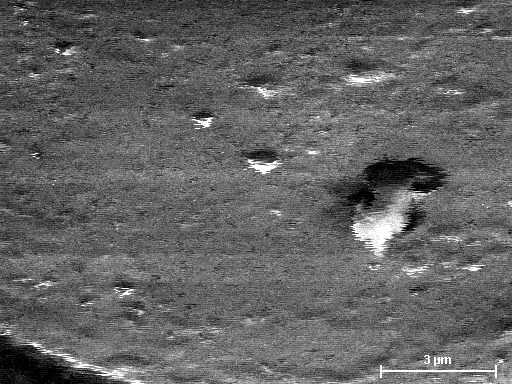
\includegraphics[width=.8\textwidth]{raw/SEM/Hummelauge_M9010}
			\subcaption{}
			\label{fig:Hummelaugex9010}
		\end{subfigure}
		\begin{subfigure}[c]{.45\textwidth}
			\centering
			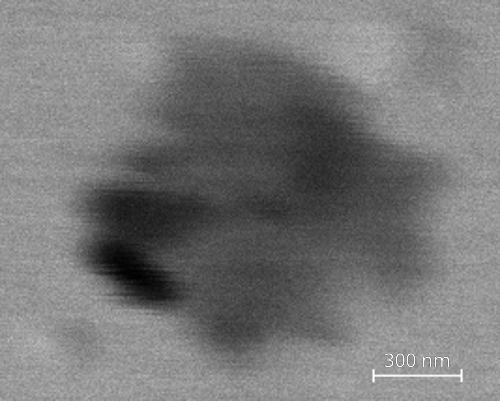
\includegraphics[width=.8\textwidth]{raw/SEM/45kresolutionExt2.png}
			\subcaption{}
			\label{fig:45k}
		\end{subfigure}
		\caption{(a) SEM-Bild eines Hummelauges bei einer Vergrößerung von x9010.\\
		(b) SEM-Bild einer für diesen Versuch hergestellten Probe bei einer Vergrößerung von x45000.
		}
		\label{fig:resolution}
	\end{figure}
	Bei einem Vergrößerungsfaktor von über $9000$ liegen diese Strukturen im \SI{1}{\micro\meter}-Bereich.
	Zum Vergleich mit geringeren Vergrößerungen dient \cref{fig:Hummelauge} im Anhang.

	\

	Um noch kleinere Strukturen mit dem SEM darzustellen, werden die für diesen Versuch hergestellten Proben verwendet.
	Lassen die Goldcluster sich auflösen, so bedeutet dies, dass die Auflösungsgrenze des SEMs in den \SI{10}{\nano\meter}-Bereich reicht.
	\cref{fig:45k} zeigt die kleinste darstellbare Struktur auf dem Kohlenstoffhintergrund der Probe.
	Goldcluster lassen sich nicht erkennen und vermutlich handelt es sich auch hier um Schmutz.
	Dennoch kann durch den Kontrast an der dunkleren Stelle mit dem umliegenden Gebiet eine Struktur im \SI{300}{\nano\meter}-Bereich erkannt werden.


\subsection{Untersuchung einer Messingprobe}

	Die zu untersuchende Messingprobe befindet sich wie auch die Kupfer- und die Zinkprobe an verschiedenen Stellen der gleichen Halterung.
	Dies ist in \cref{fig:messing_halterung} dargestellt.
	\begin{wrapfigure}{r}{.5\textwidth}
		\centering
		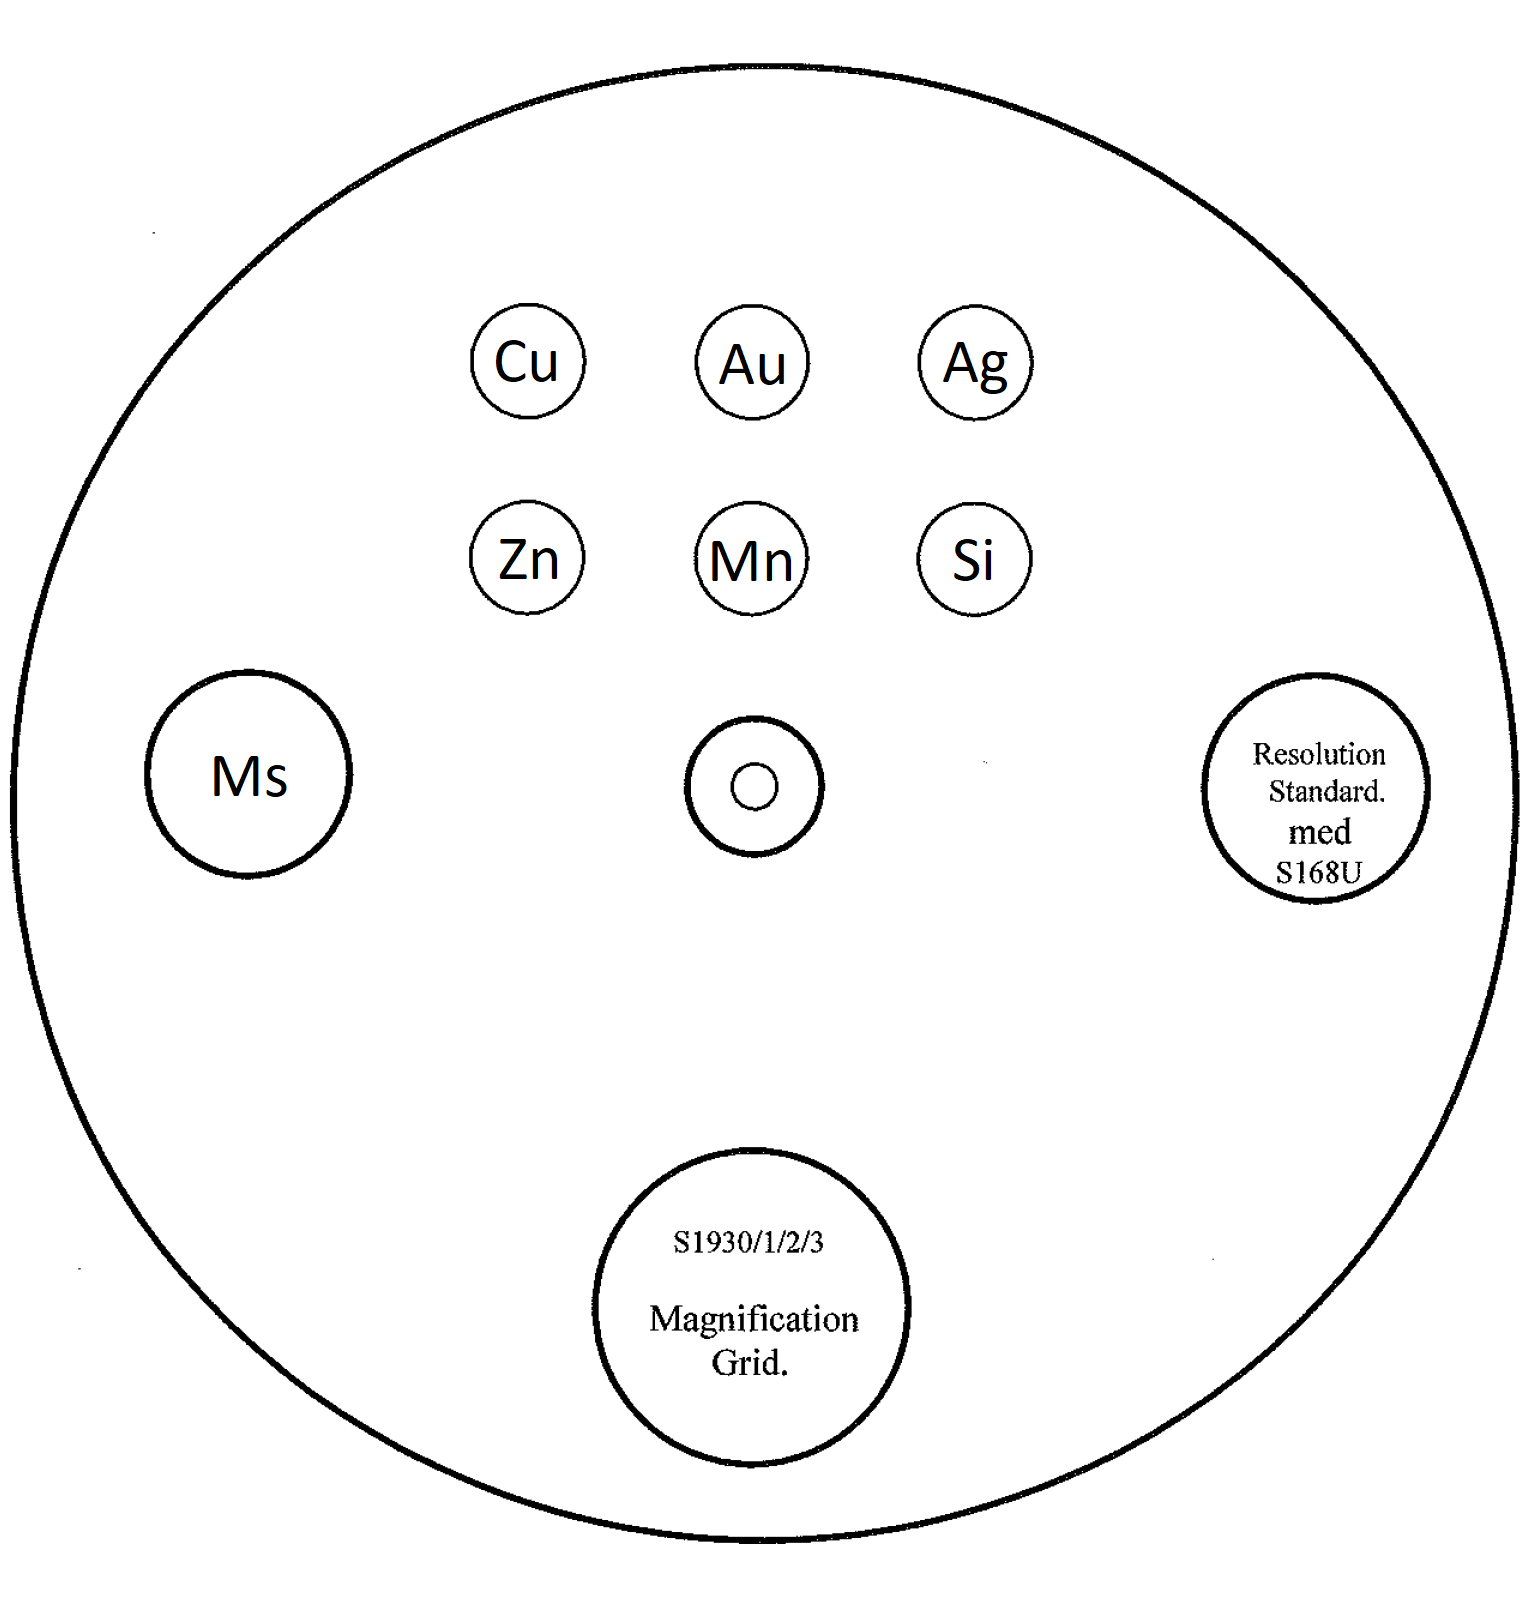
\includegraphics[width=.4\textwidth]{img/Messingprobe}
		\caption{Schematische Darstellung der Halterung mit unterschiedlichen Proben.\cite{wwu}}
		\label{fig:messing_halterung}
	\end{wrapfigure}
	Um nur das Röntgen-Absorptionsspektrum einer bestimmten Probe aufzunehmen, wird nur der Bereich, welcher von Interesse ist, abgebildet.
	Dafür wird die zu untersuchende Probe innerhalb des Mikroskops in den Mittelpunkt des Elektronenstrahls gefahren und die Vergrößerung erhöht, damit nur eine Legierung bzw. ein Element sichtbar ist.

	\

	In \cref{fig:messing_spektrum} sind die aufgenommen Spektren für Messing, Kupfer und Zink zu erkennen.
	Da für die Bestimmung von Kupfer- und Zinkgehalt hier nur die charakteristischen $K_\alpha$- und $K_\beta$-Linien relevant sind, sind die gesamten Spektren und Darstellungen der $L$-Linien (\cref{fig:l-linien}) dem Anhang zu entnehmen.
	Letztere sind für die Auswerung nicht geeignet, da dort nicht zwischen $L_\alpha$ und $L_\beta$ unterschieden werden kann.

	Die Verteilung der Datenpunkte um die $K$-Linien werden als gaußförmig angenommen und daher mit Gauß-Funktionen angenähert.
	Als Startparameter dienen die von \cite{brukerPTE} gegebenen Energien für die $K$-Linien von Kupfer und Zink.
	Dargestellt ist dies in \cref{fig:k-linien}.
	\begin{figure}[ht]
		\centering
		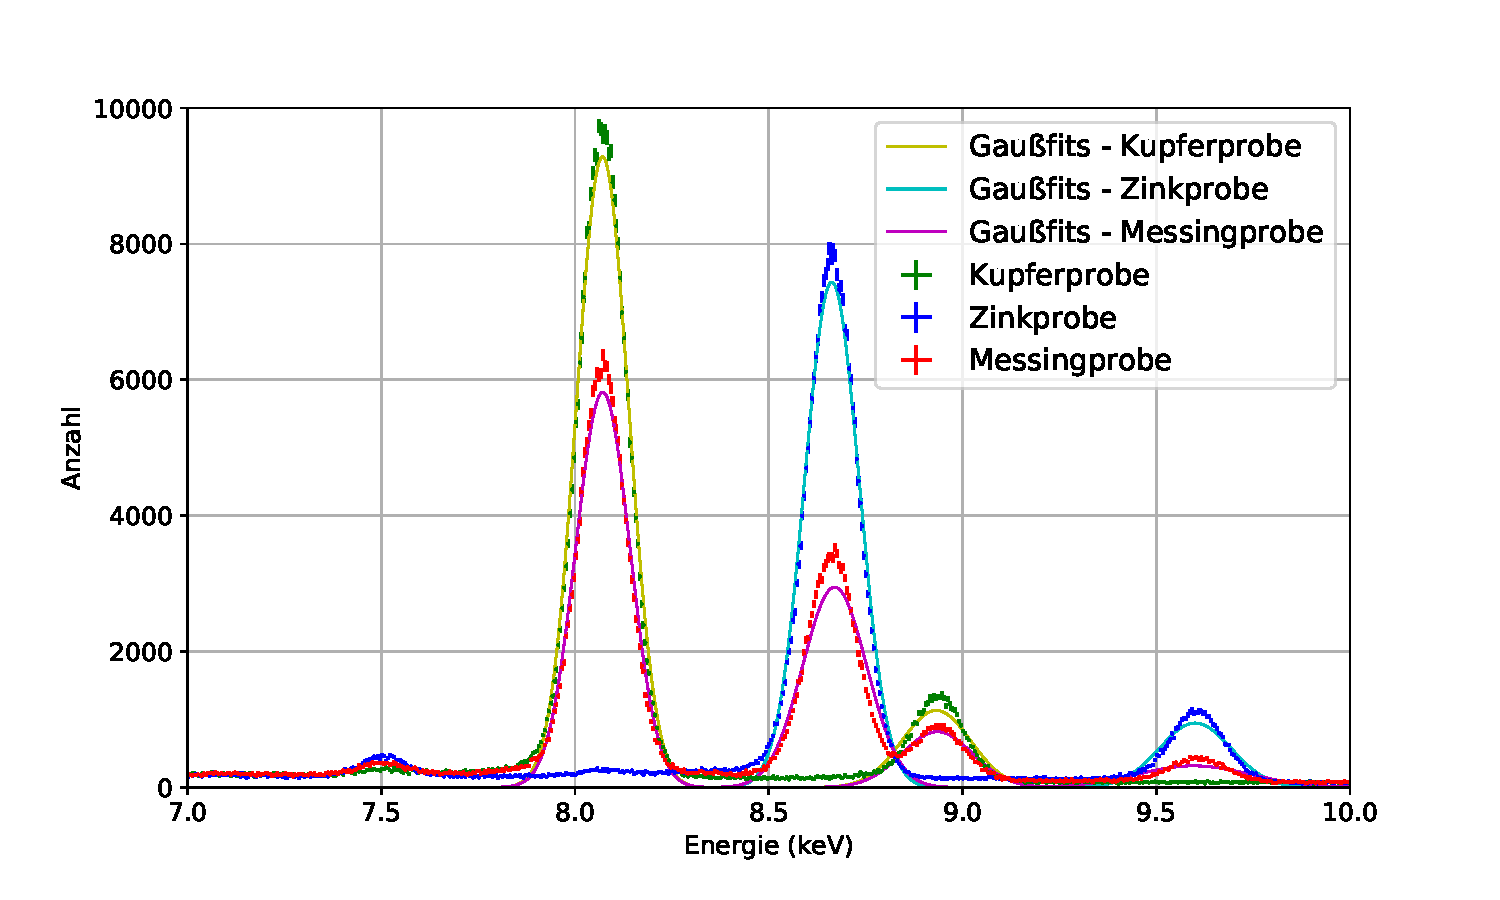
\includegraphics[width=.8\textwidth]{plots/KupferprobeK}
		\caption{Röntgen-Absorptionsspektrum im Bereich der $K$-Linien von Kupfer und Zink für eine Messing-, Kupfer- und Zinkprobe. Zusätzlich dazu Gauß-Fits für die einzelnen Proben und deren charakteristischer Linien.}
		\label{fig:k-linien}
	\end{figure}
	Für die Unsicherheit der Anzahl von $n$ Datenpunkten wird $\sqrt{n}$ verwendet.
	Der direkte Vergleich der Amplituden der Gauß-Fits von Messing zu denen von Kupfer bzw. Zink liefert die in \cref{tab:amplituden} dargestellte Verhältnisse.
	\begin{table}[H]
		\centering
		\caption{Verhältnisse der Amplituden charakteristischer Linien von Messing (Ms) zu Kupfer (Cu) bzw. Zink (Zn).}
		\begin{tabular}{l|c|c|c}
			Verhältnis & $K_\alpha$ & $K_\beta$ & Mittelwert \\ \hline
			% & & & \\
			Ms/Cu & $(62.6\pm3.5)\%$ & $(72.0\pm9.0)\%$ & $(67.0\pm5.0)\%$ \\
			Ms/Zn & $(39.6\pm2.9)\%$ & $(34.0\pm4.0)\%$ & $(36.6\pm2.5)\%$ \\
		\end{tabular}
		\label{tab:amplituden}
	\end{table}

\subsection{Untersuchung unbekannter Elemente}

	Für die letzte SEM-Messung wird die Probe mit den vier unbekannten Elementen eingesetzt.
	Um die Elemente zu bestimmen, wird zunächst ein Bild von jedem Quadranten aufgenommen und das zugehörige Röntgen-Absorptionsspektrum betrachtet.
	Die Software von Bruker ermöglicht einen direkten Vergleich der aufgenommenen Spektren mit den Absorptionslinien einer Vielzahl an Elementen.
	Die größte Übereinstimmungen ergeben sich bei den Elementen Aluminium, Kupfer, Silber und Kohlenstoff.

	Um eine Karte der Elemente anzufertigen, wird ein Bild der Probenmitte aufgenommen.
	Bei jedem Rastervorgang wird pro Position ein Spektrum aufgenommen und direkt mit den ausgewählten Elementen verglichen.
	Wie in \cref{fig:bunteMap} dargestellt, nimmt ein Pixel bei Übereinstimmung die Farbe des jeweiligen Elements an.
	\begin{figure}[H]
		\centering
		\begin{subfigure}[c]{.45\textwidth}
			\centering
			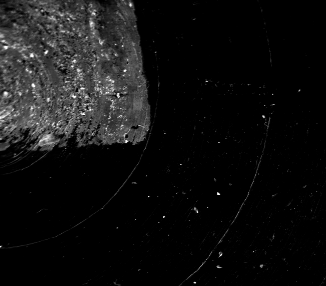
\includegraphics[width=.8\textwidth]{raw/SEM/Map4ProbenExt}
			\subcaption{}
			\label{fig:farbloseMap}
		\end{subfigure}
		\begin{subfigure}[c]{.45\textwidth}
			\centering
			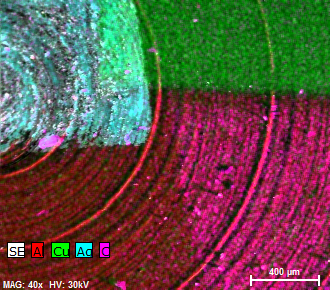
\includegraphics[width=.8\textwidth]{raw/SEM/Mapdaten4Proben}
			\subcaption{}
			\label{fig:bunteMap}
		\end{subfigure}
		\caption{(a) SEM-Bild der Proben mit den unbekannten Elementen.
		(b) SEM-Bild mit Elementkarte aus den Röntgen-Absorptionsspektren von Silber, Kupfer, Aluminium und Kohlenstoff.}
		\label{fig:elementalMap}
	\end{figure}
	Ohne die Röntgenanalyse lassen sich drei der Quadranten, wie in \cref{fig:farbloseMap} zu sehen, nicht unterscheiden.

\subsection{Diskussion der SEM-Ergebnisse}

	Zur Bestimmung der Auflösungsgrenze wurden verschiedene Proben untersucht.
	Die bestmögliche Auflösung lag im \SI{300}{\nano\meter}-Bereich.

	\

	Durch Mittelung ergab sich für den Kupfergehalt im Messing ein Wert von $(67.0\pm5.0)\%$ und für den Zinkgehalt $(36.6\pm2.5)\%$.
	Als Angabe für das Messing wurde "duplex brass" von \cite{wwu} verwendet.
	Nach \cite{wikiMs} entspricht dies Messing mit einem Kupfergehalt von 55\% bis 65\% und dementsprechend einen Zinkgehalt von 35\% bis 45\%.
	Damit liegt über die hier ermittelten Werte eine Übereinstimmung innerhalb einer Unsicherheit vor.
	Ein tatsächliches Verhältnis von ~65\% Kupfer zu ~35\% liegt nahe.
	Es sei angemerkt, dass die getrennte Betrachtung der unterschiedlichen $K$-Linien eine größere Übereinstimmung für die $\alpha$- und eine geringere für die $\beta$-Linen mit sich trägt.
	Dass die Anzahl der Datenpunkte bei den $\beta$-Linen deutlich geringer war, könnte eine mögliche Begründung dafür sein, weswegen bei einer längeren Messung möglicherweise ein besseres Ergebnis erzielt werden könnte.

	\

	Der letzte Punkt der SEM-Auswertung befasste sich mit der Erstellung der Elementkarte.
	Hier ließen sich die vier unbekannten Elemente zu Silber, Kupfer, Aluminium und Kohlenstoff bestimmen.
	Der direkte Vergleich zwischen SEM-Bild ohne und mit der Elementkarte in \cref{fig:elementalMap} unterstützt dies.
	Ohne die Elementkarte sticht nur ein Element hervor.
	Aus der Röntgenanalyse folgt, dass es sich dabei um Silber handelt.
	Dies erscheint sinnvoll, da Silber von den vier Elementen die höchste Ladungszahl besitzt, somit eine Wechselwirkung mit den Strahlelektronen am wahrscheinlichsten ist und daher im SEM-Bild am hellsten erscheint.
	Weiterhin kann \cref{fig:bunteMap} entnommen werden, dass die Probe eine Aluminiumbasis besitzt, auf die andere Elemente aufgedampft wurden.
	Besonders an dem Kohlenstoffquadranten ist dies ersichtlich, da neben den pinken Pixeln auch rote vorliegen.
	Ebenso grenzt der Kupferquadrant nicht direkt an den Kohlenstoff, sondern es befindet sich noch Aluminium dazwischen.
